\documentclass{beamer}

\mode<presentation>

\usetheme{Pittsburgh}


\usepackage[utf8]{inputenc}
\usepackage{ beamerthemesplit}
\usepackage{caption}
\usepackage{adjustbox}
\newtheorem*{defi}{Definición}
\newtheorem*{teor}{Teorema}
\newtheorem*{teort}{Teorema de Tibor Radó}
\newtheorem*{lema}{Lema}
\newtheorem*{ejem}{Ejemplos}
\newtheorem*{prop}{Proposición}

%\mode<handout>
{
\beamertemplatesolidbackgroundcolor{black!5}
}
\usepackage{amssymb,amsmath,amsfonts,graphicx,float,epsfig,enumerate}
\usepackage{amsopn}
\usepackage{fancyhdr}
\renewcommand{\figurename}{Figura}

\renewcommand{\baselinestretch}{1}

% \newenvironment{flushenum}{
% \begin{enumerate}
%   \setlength{\leftmargin}{0pt}
% }{\end{enumerate}}

\sloppy

\parindent 0pt

%\usepackage[dark,tab]{beamerthemesidebar}

%\logo{\includegraphics[width=1cm,height=1cm]{logo.pdf}}

\title[Teorema de clasificación de superficies]{Teorema de clasificación de superficies topológicas}
\author[Rodrigo De Pool]{}
%\institute[UAM]{}
\date[]{Junio 2020}
\subject{}

%\AtBeginSubsection[]
%{
% \begin{frame}<beamer>
%    \frametitle{Plan of the talk}
%    \tableofcontents[currentsection,currentsubsection]
%  \end{frame}
% }

\newcommand{\oo}{$^{\mbox{\underline{\tiny o}}}$\hspace{2 mm}}

\definecolor{dark}{gray}{.5}
\definecolor{rosa_claro}{rgb}{1,0.9,0.9}
%\definecolor{azul_intenso}{rgb}{0,0.6,0.9}
\definecolor{azullito}{rgb}{0.4,0.5,0.9}
%\definecolor{amarillo_claro}{rgb}{1,1,0.7}
%\definecolor{gris_claro}{gray}{0.9}
\definecolor{uofsgreen}{rgb}{.125,.5,.25}

\usecolortheme[named=azullito]{structure} % Para cambiar el fondo de los frametitles

\begin{document}
%%%%%%%%%%%%%%%%%%%%%%%%%%%%%%%%%%%%%%%%%%%%%%%%%%%%%%%%%%%%%%%%%%%%%%%%%%%%%
%%%%% TITULO %%%%%%%%%
\frame{\titlepage}
 
%%%%%% DIAPOSITIVA 2 %%%%%%
\begin{frame}
\frametitle{Superficies topológicas}

\begin{defi}
S es superficie topológica si
\begin{itemize}
    \item Localmente homeomorfo a una bola en $\mathbb{R}^2$.
    \item Hausdorff, segundo numerable y conexo (*orientable).
\end{itemize}
\end{defi}

\begin{figure}[htb]
\begin{center}
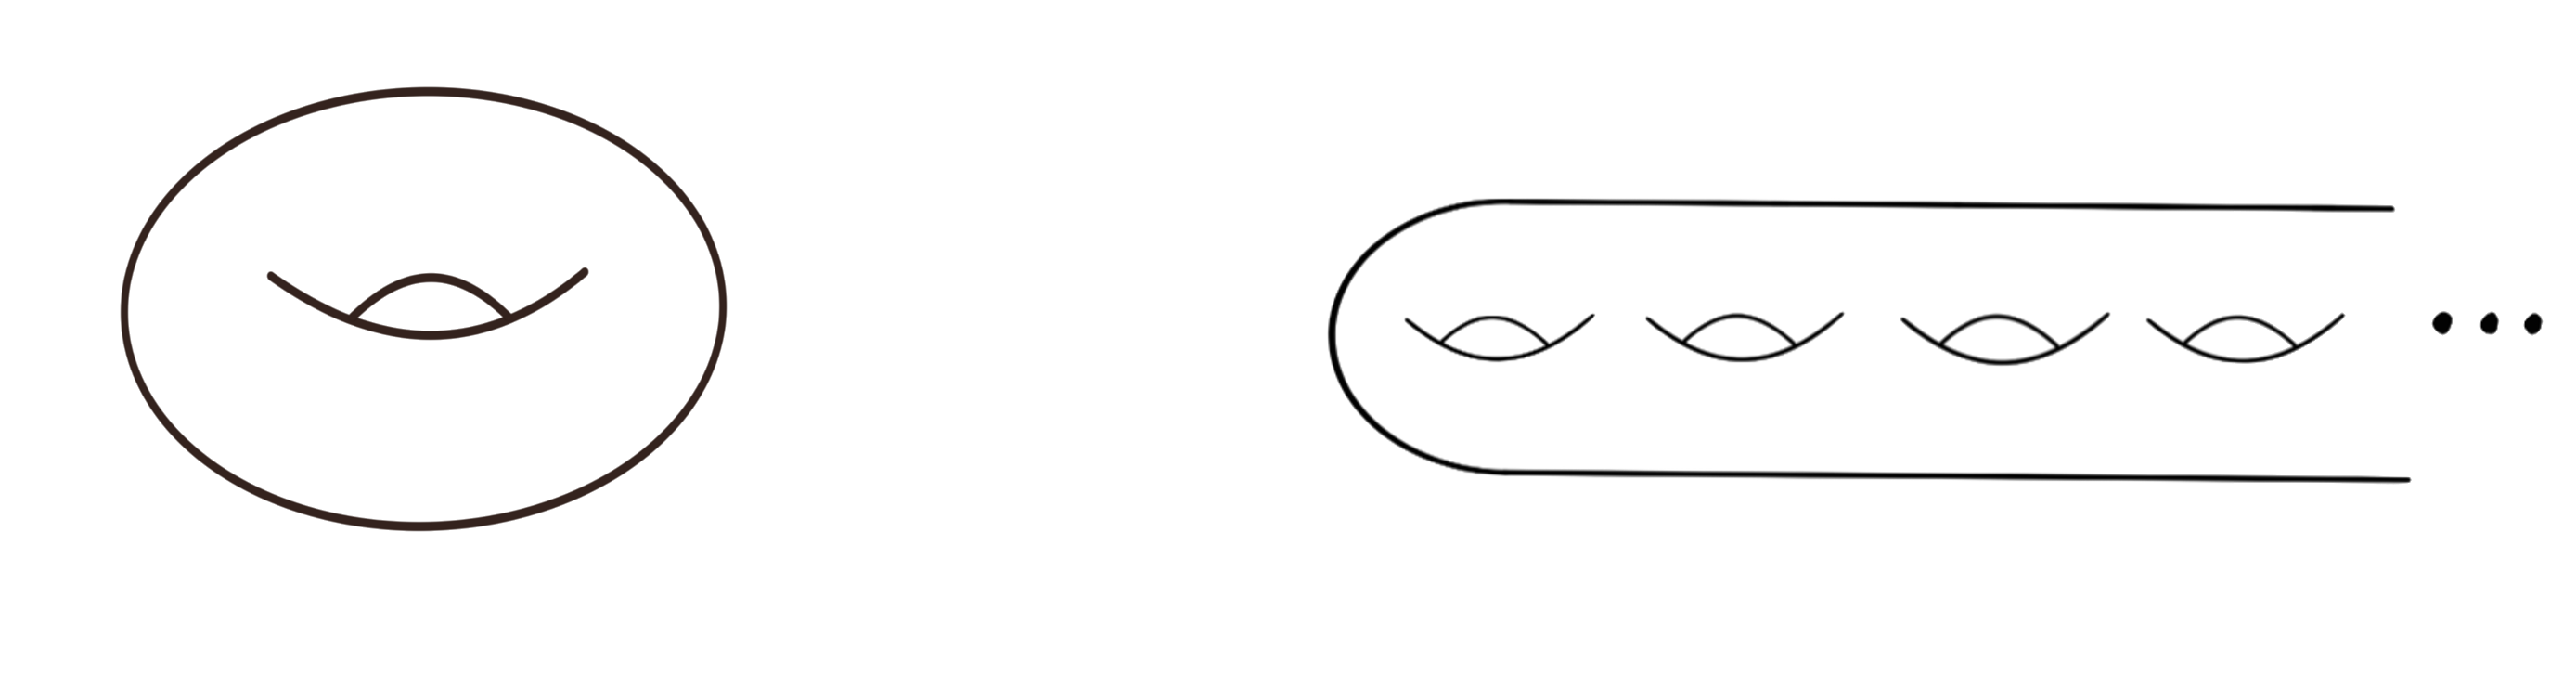
\includegraphics[width=3in,height=1in]{imagenes/diapo1.png} 
\caption{Una superficie compacta y otra no compacta}
\end{center}
\end{figure}

\end{frame}

%%%%%% DIAPOSITIVA 4 %%%%%%
\begin{frame}
\frametitle{Suma conexa}

\begin{defi}
La suma conexa es un operador entre superficies:
\[S' = S_1 \# S_2 \]
$S'$ resulta de de retirar un disco abierto de cada superficie e identificarlas por el borde.
\end{defi}

\begin{figure}[htb]
\begin{center}
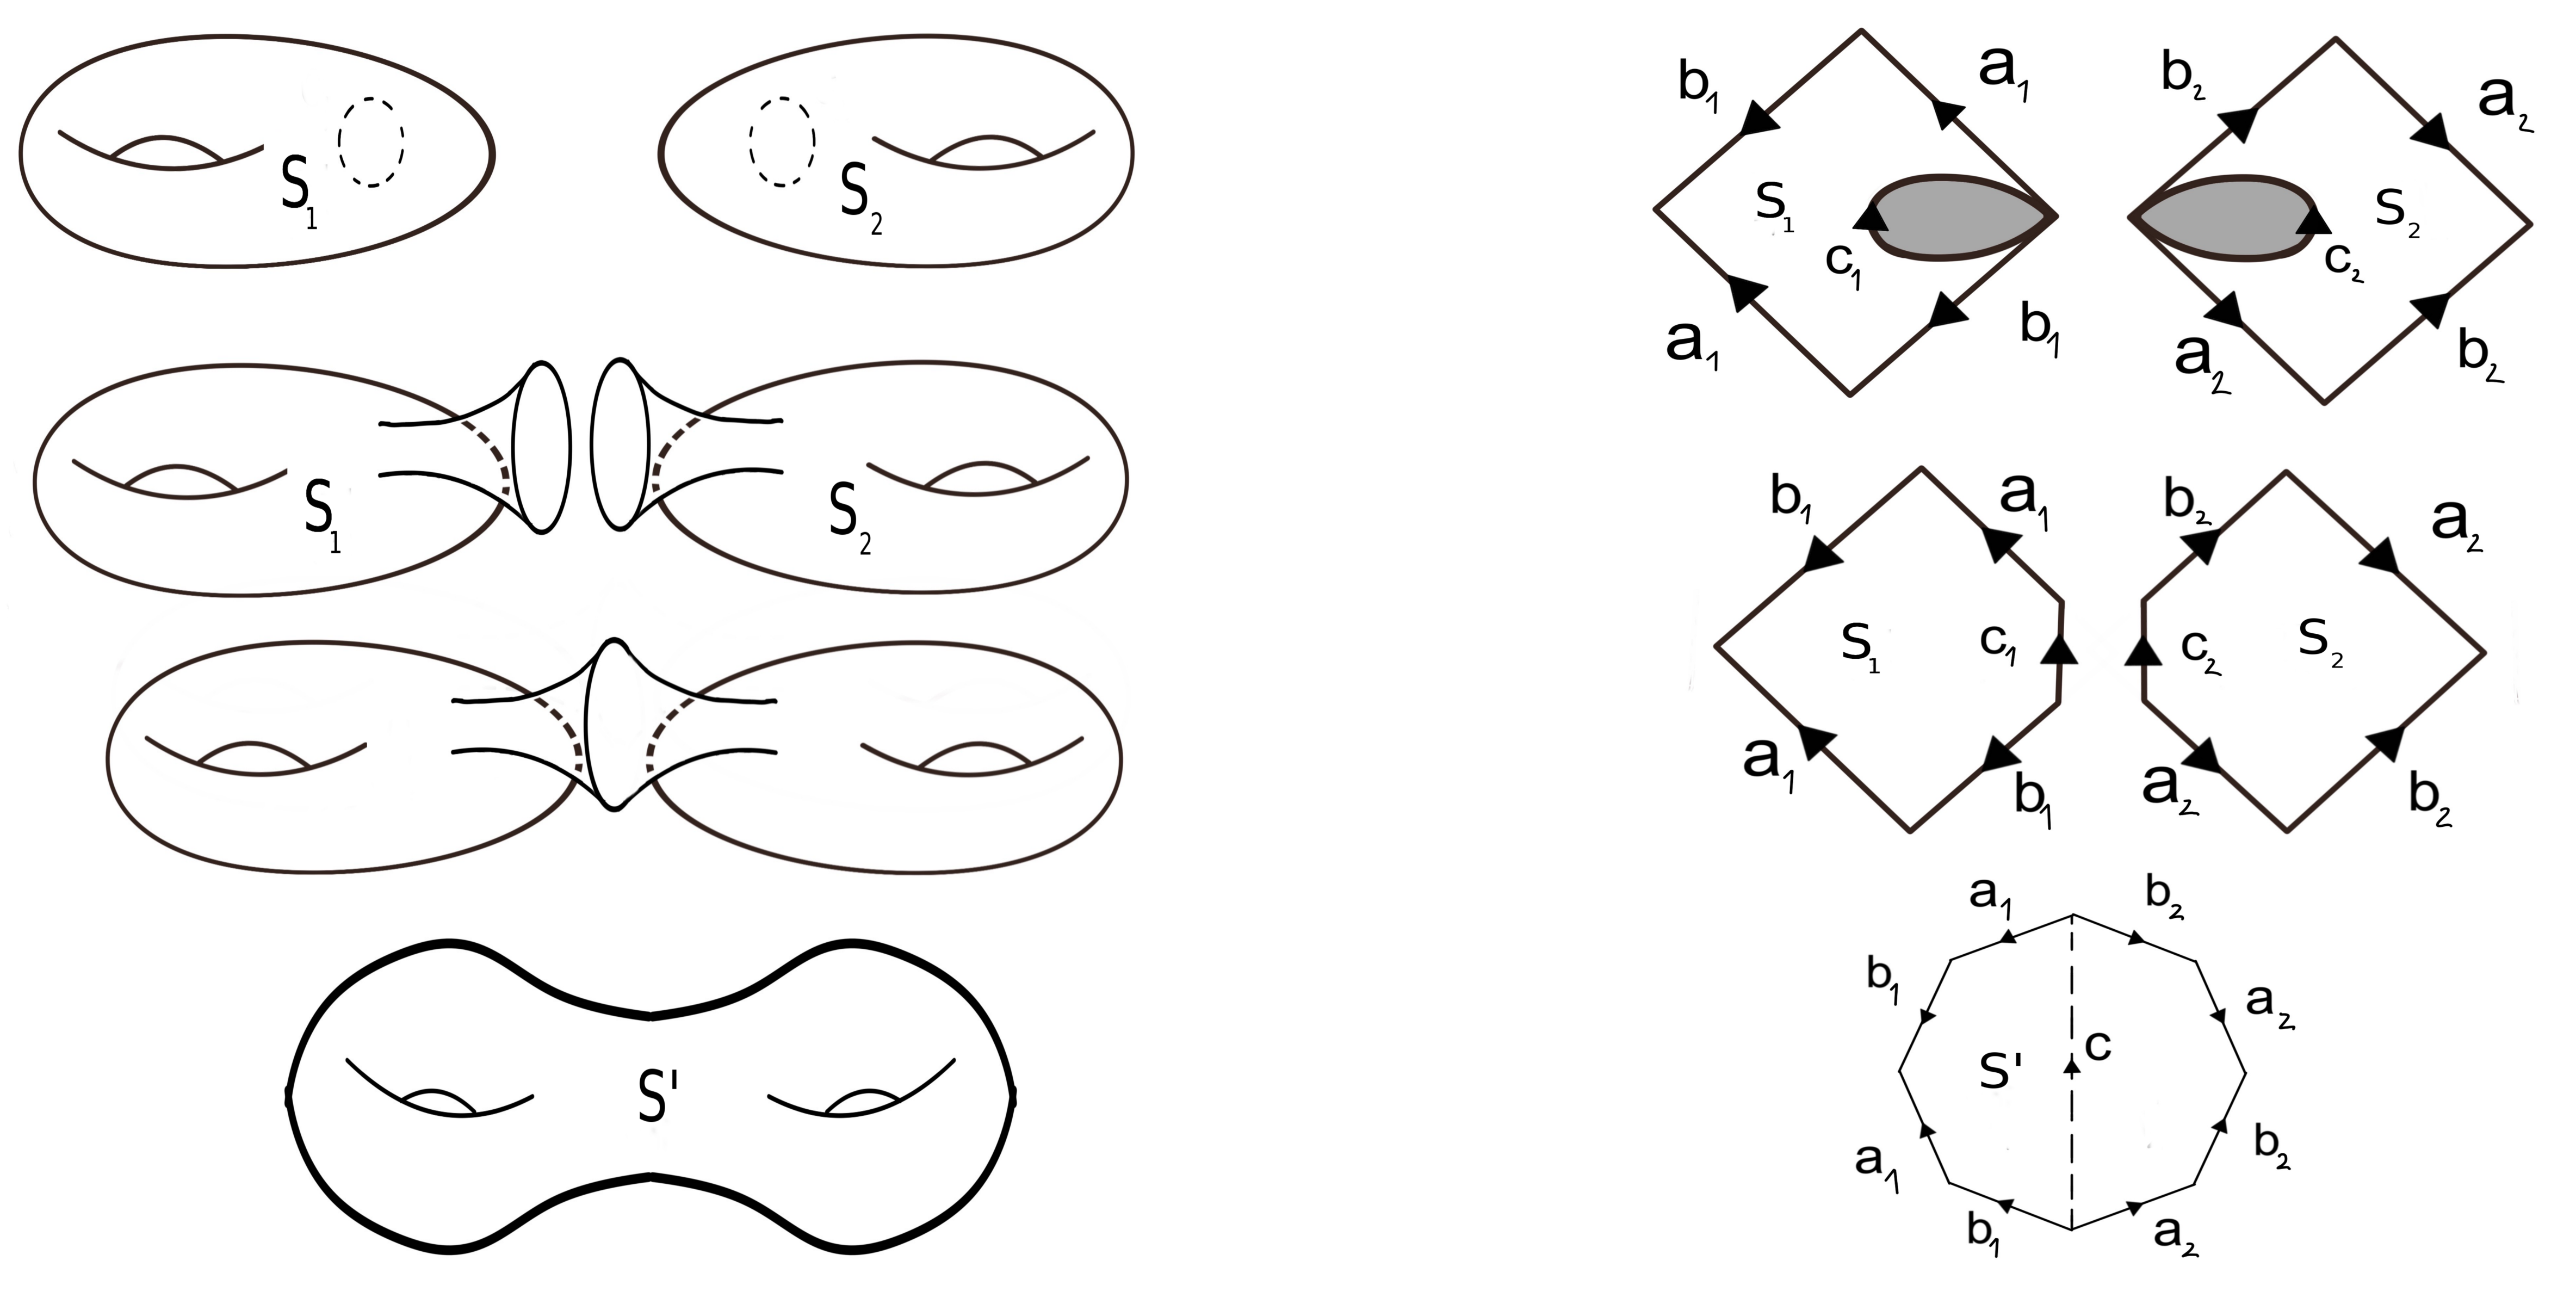
\includegraphics[width=3in,height=1.5in]{imagenes/diapo2.png} 
\caption{Suma conexa de toros}
\end{center}
\end{figure}

\end{frame}


%%%%%% DIAPOSITIVA 6 %%%%%%
\begin{frame}
\frametitle{Triangulación de una superficie}


\begin{defi}
Una triangulación de una superficie S es una colección de subconjuntos cerrados $\{T_1, T_2, ..., T_n\}$ que recubren a la superficie y cumplen:
\begin{itemize}
\item Todo $T_i$ es homeomorfo a un triangulo en $\mathbb{R}^2$.
\item Dos conjuntos $T_i$ y $T_j$ distintos o son disjuntos o comparten solo un vértice o comparten toda una arista.
\end{itemize}

\end{defi}
\end{frame}

%%%%%% DIAPOSITIVA 7 %%%%%%
\begin{frame}

\frametitle{Triangulación}
\begin{ejem}
Toro y esfera triangulados
\begin{figure}[htb]
\begin{center}
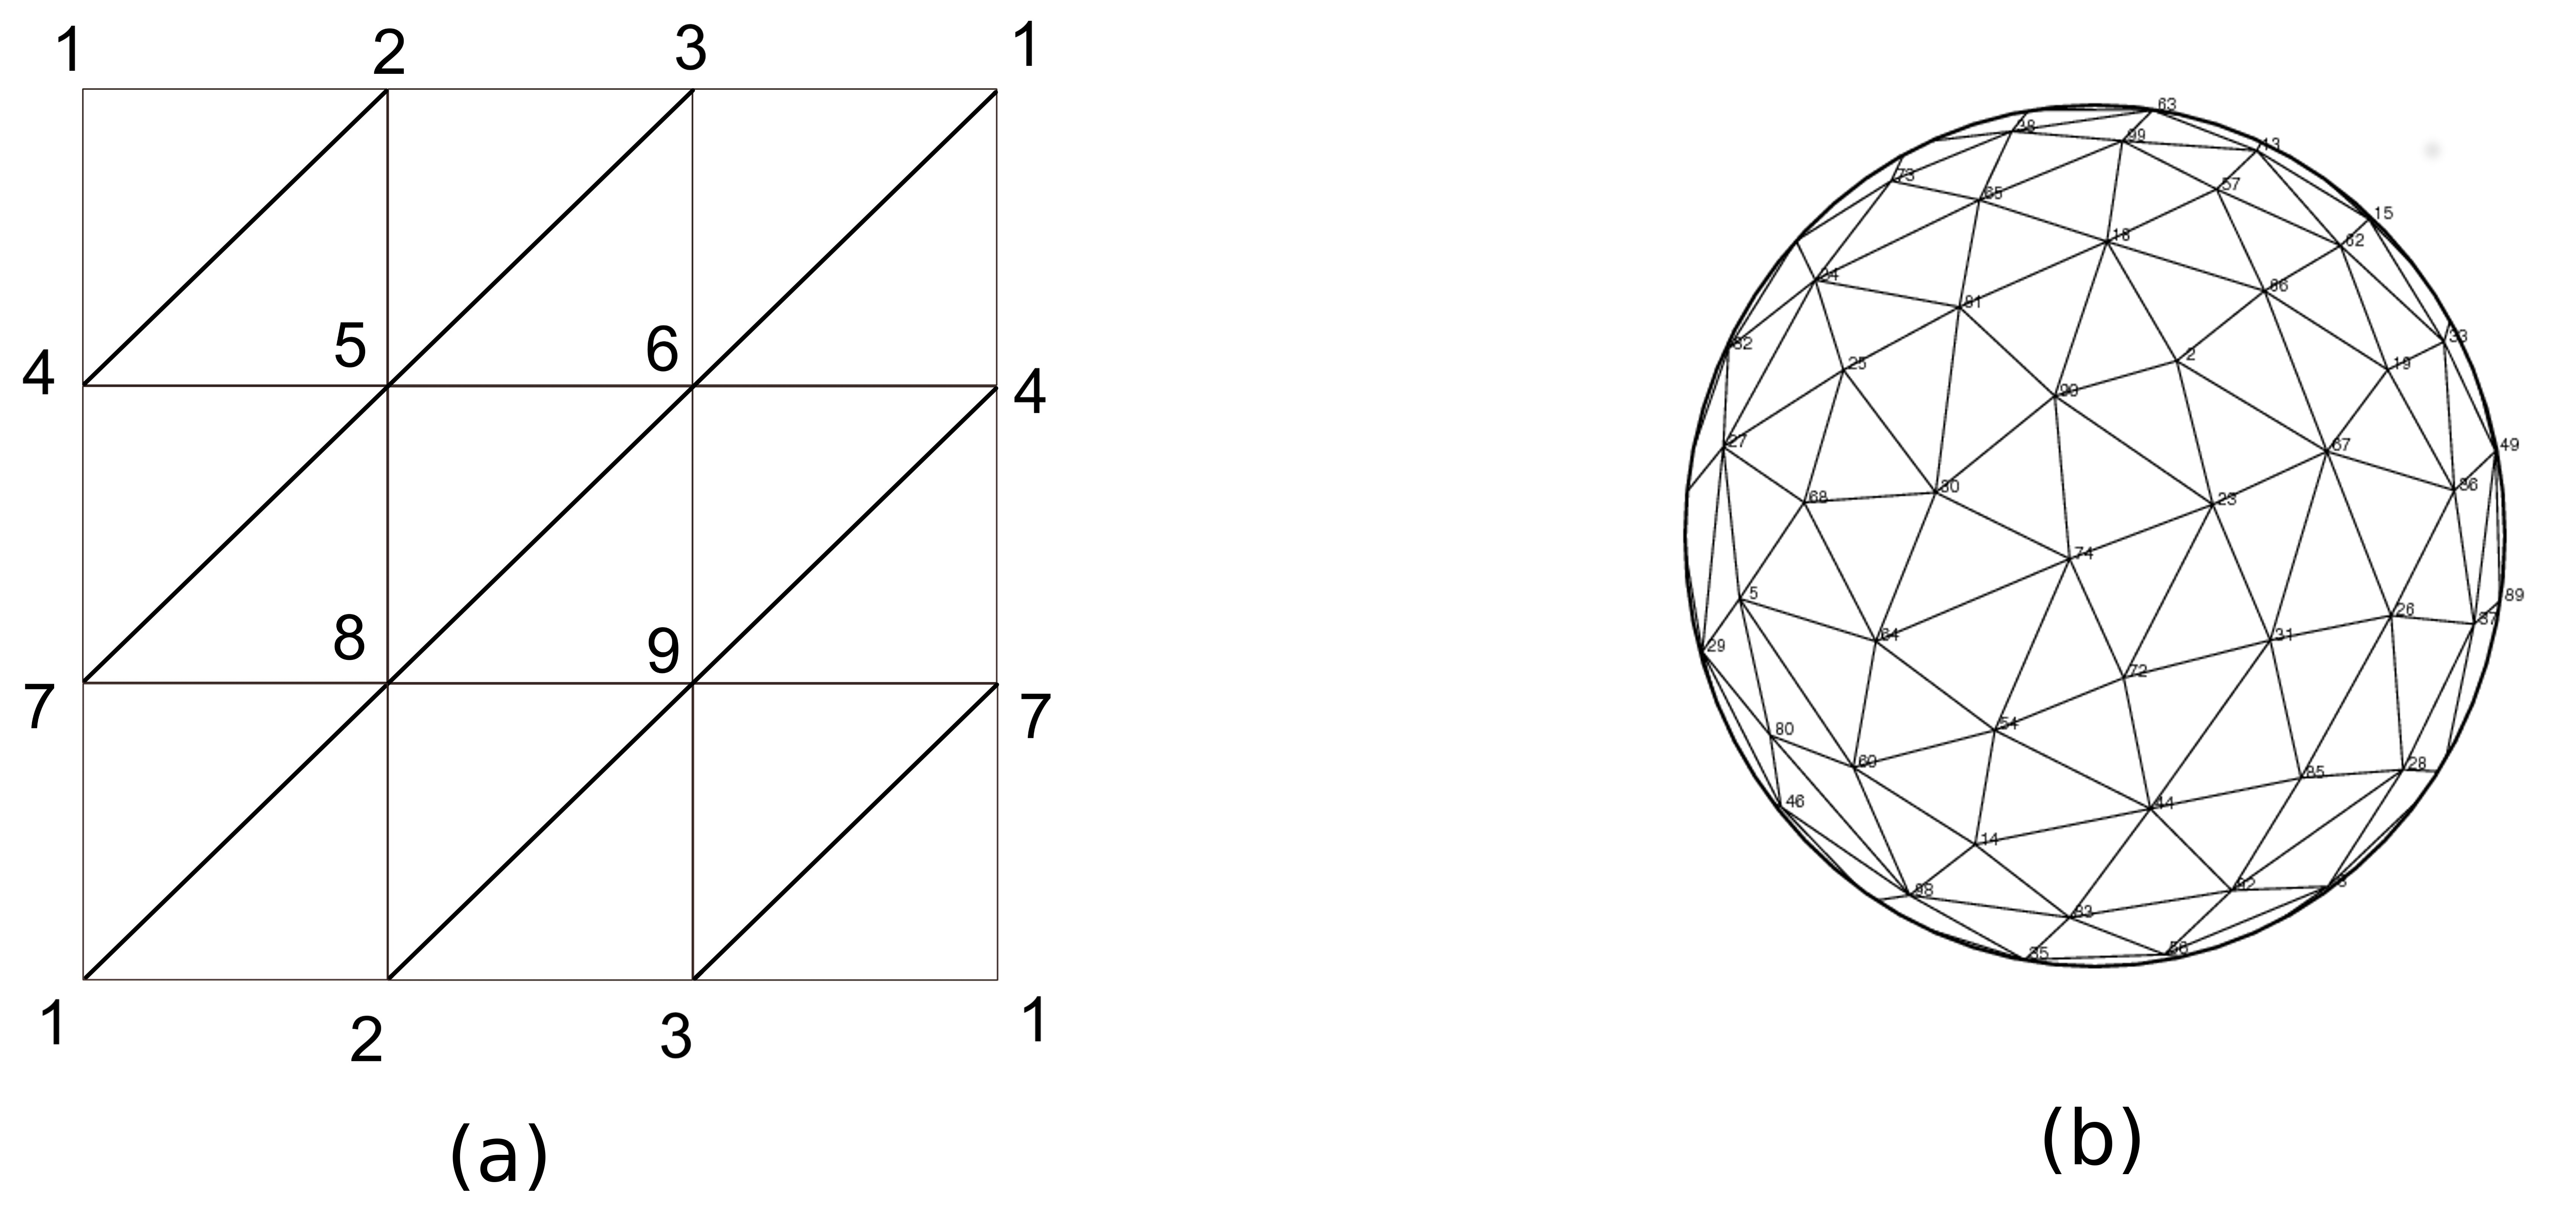
\includegraphics[width=2in,height=0.75in]{imagenes/diapo3.png} 
\end{center}
\end{figure}

\end{ejem}

\begin{teort}
Toda superficie separable es triangulable.
\end{teort}


\end{frame}

%%%%%% DIAPOSITIVA 8 %%%%%%
\begin{frame}
\frametitle{Teorema de clasificación de superficies compactas}
\begin{teor}
Toda superficie compacta orientable es homeomorfa o a una esfera o una suma conexa de $n$ toros.
\end{teor}
\begin{figure}[htb]
\begin{center}
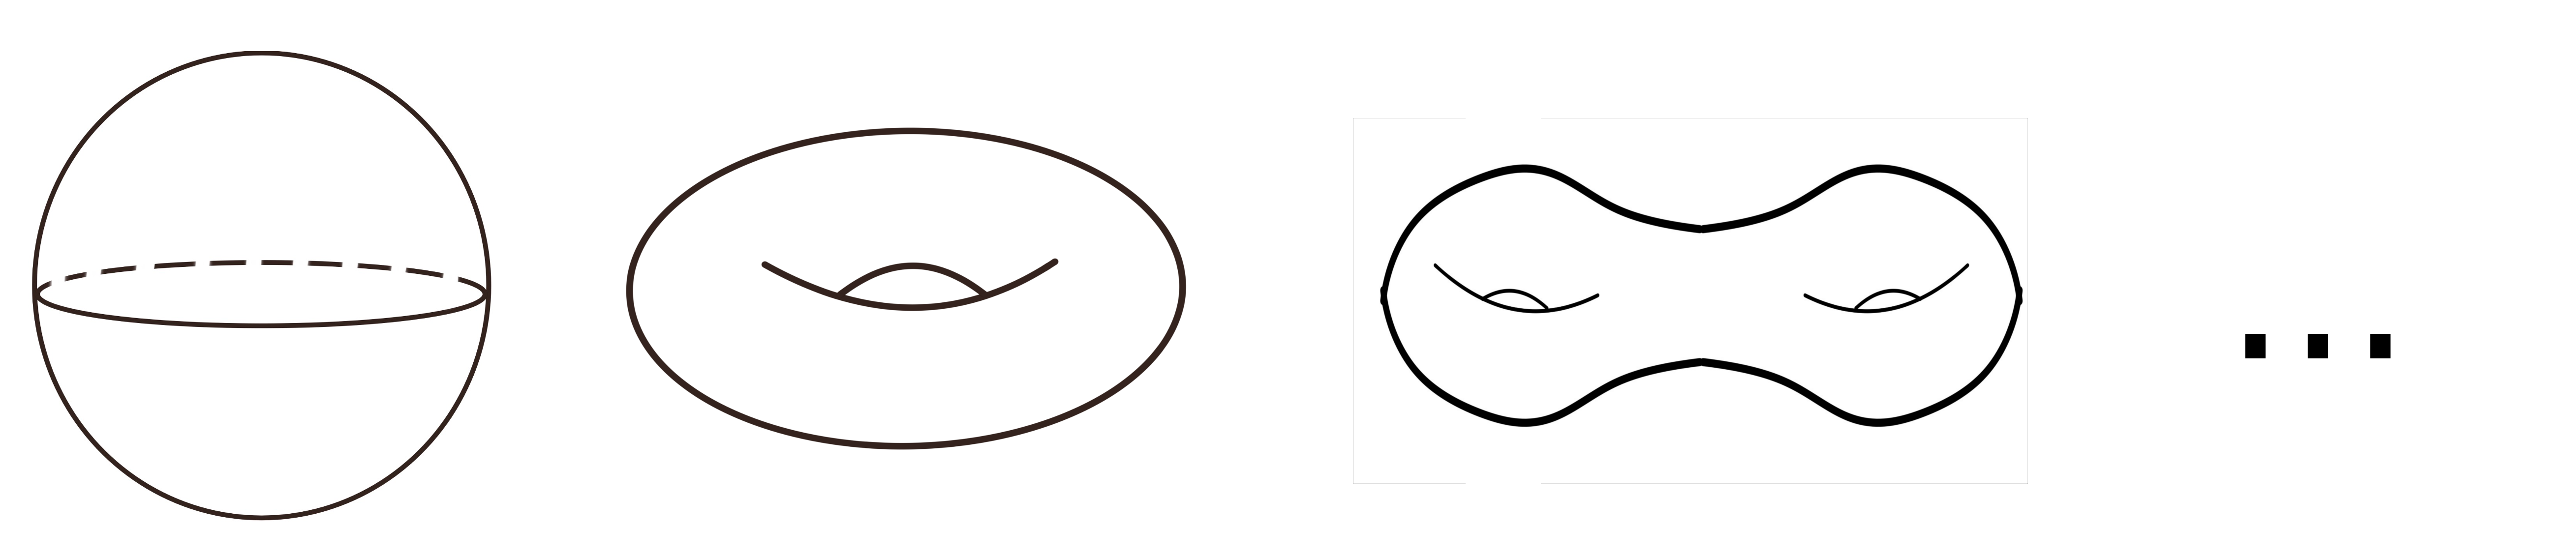
\includegraphics[width=4in,height=0.75in]{imagenes/diapo4.png} 
\end{center}
\end{figure}

\end{frame}

%%%%%% DIAPOSITIVA 9 %%%%%%
\begin{frame}
\frametitle{Demostración}
\begin{proof}[Demostración]
Primero, se utiliza el teorema de Tibor Radó para expresar una superficie como un polígono donde todas las aristas del borde están identificadas a pares.

Luego, mediante cortes e identificaciones obtenemos un nuevo polígono que es equivalente o a una esfera o una suma conexa de $n$ toros.

\begin{figure}[htb]
\begin{center}
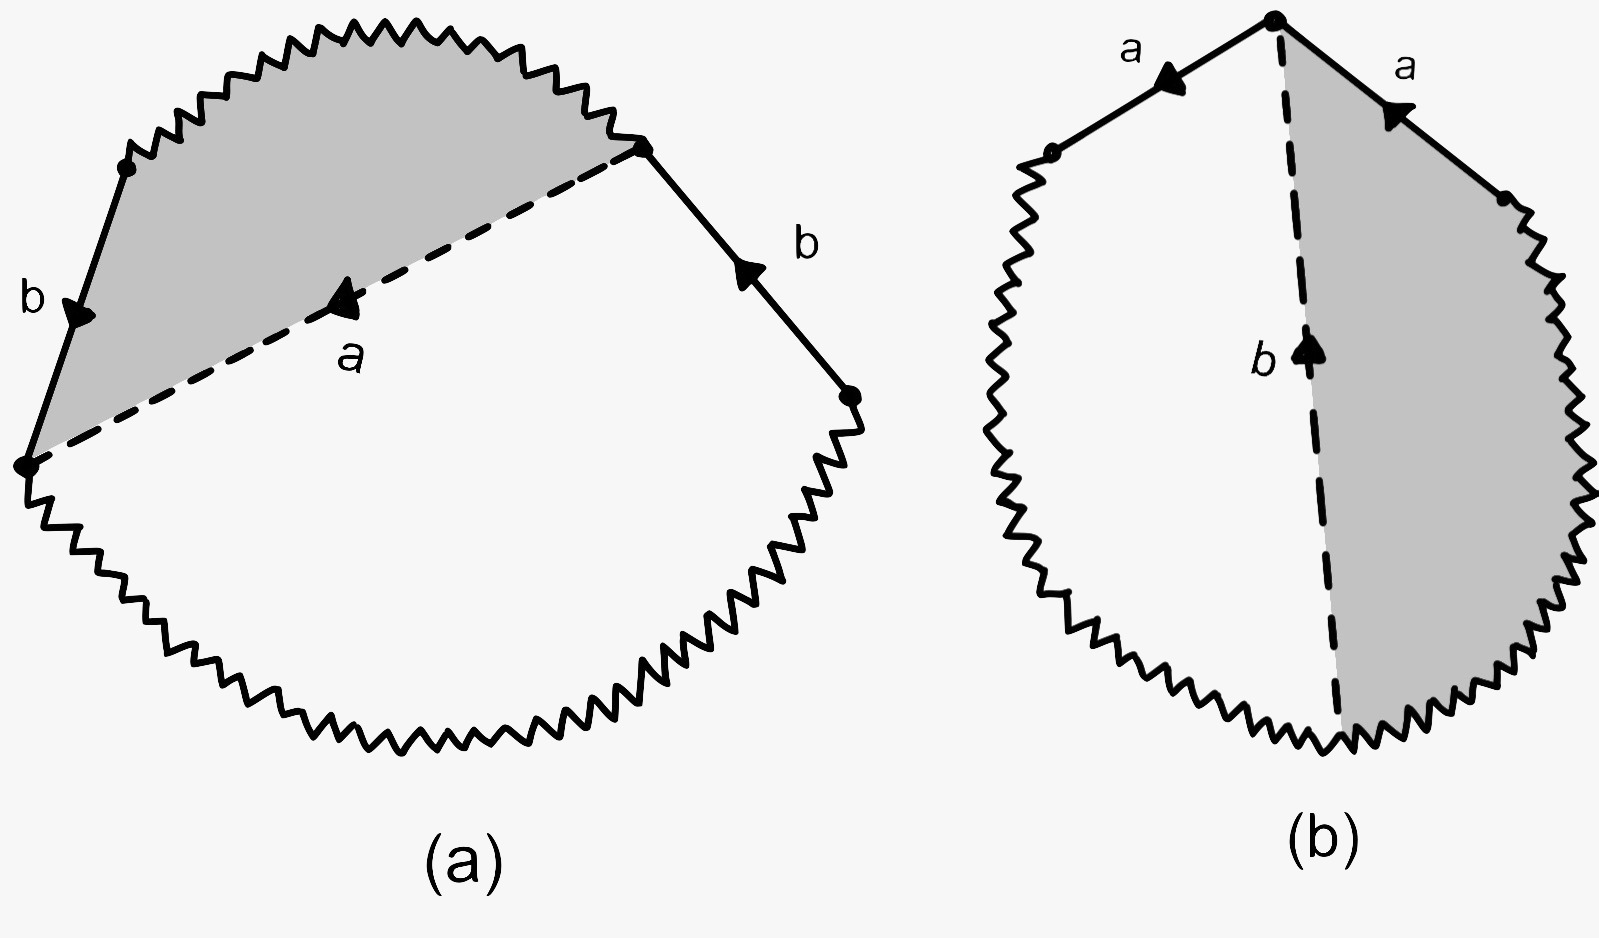
\includegraphics[width=2in,height=0.75in]{imagenes/paso4.jpeg} 
\caption{recorte e identificación}
\end{center}
\end{figure}
 
\end{proof}

\end{frame}

%%%%%% DIAPOSITIVA 10 %%%%%%
\begin{frame}
\frametitle{Género}
\begin{figure}[htb]
\begin{center}
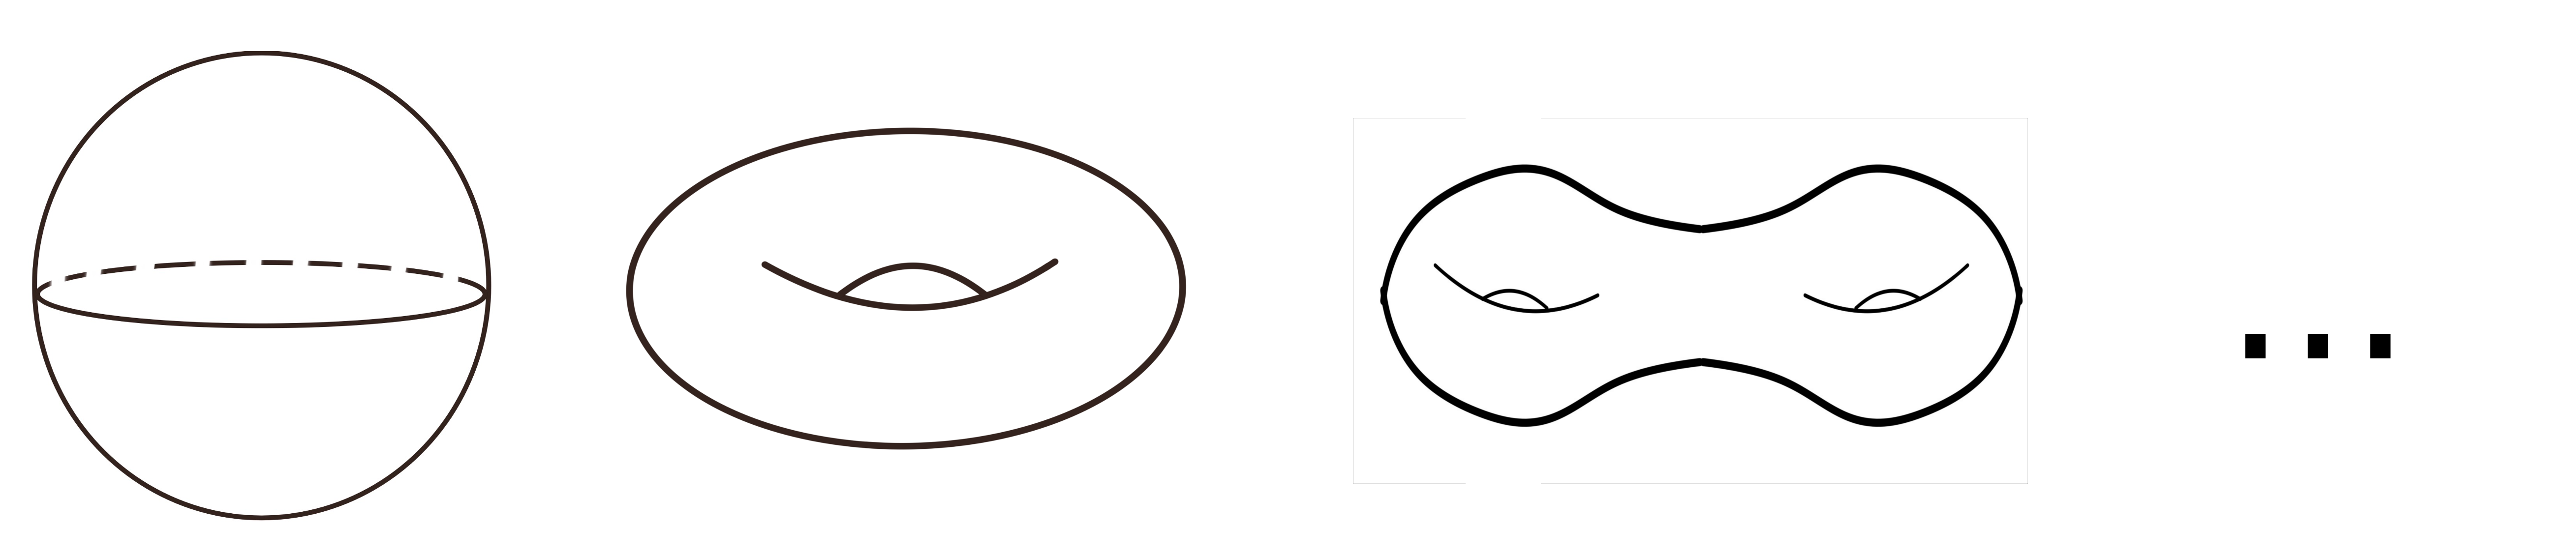
\includegraphics[width=4in,height=0.75in]{imagenes/diapo4.png} 
\end{center}
\end{figure}

Llamaremos \textit{género} de una superficie compacta al número $n$ de toros al que es homeomorfa. Si es homeomorfa a una esfera diremos que tiene género 0.

\end{frame}

%%%%%% DIAPOSITIVA 11 %%%%%%
\begin{frame}
\frametitle{Clasificación de superficies no compactas}

Superficies no compactas:
\begin{figure}[htb]
\begin{center}
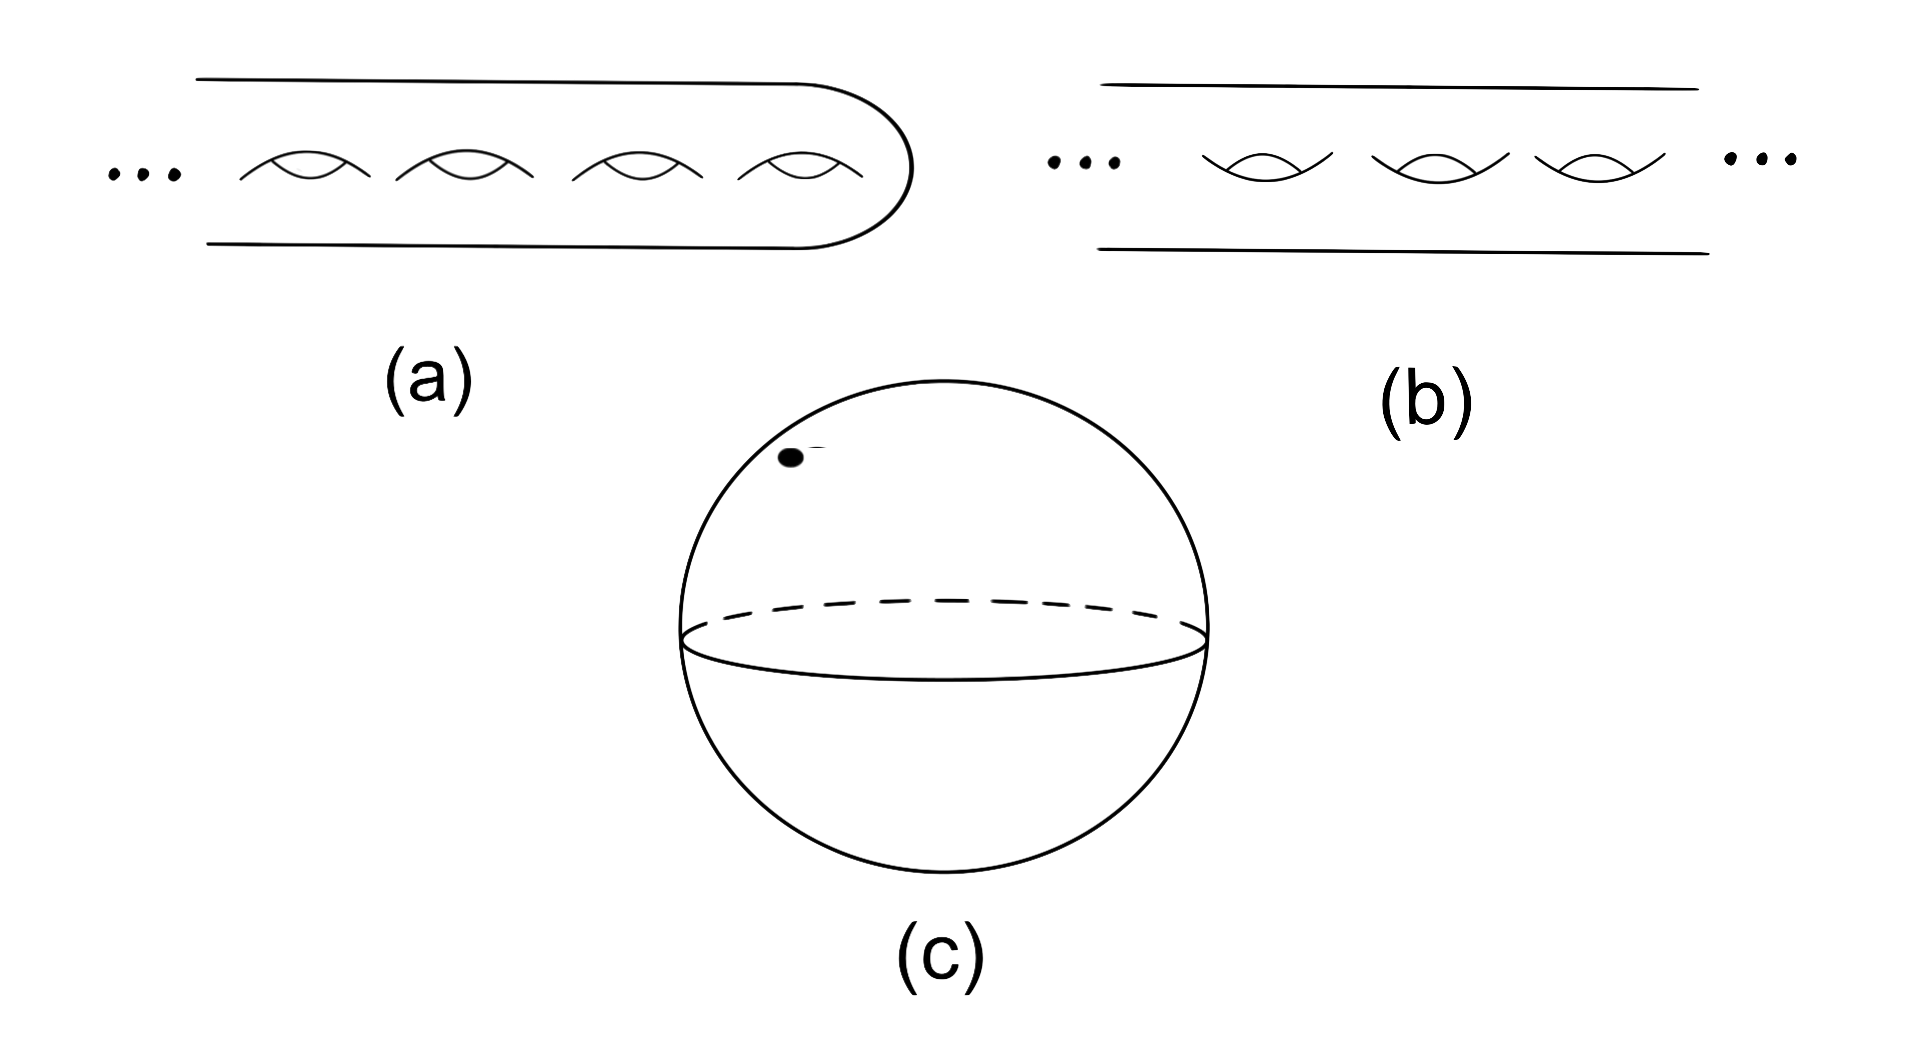
\includegraphics[width=3in,height=1.25in]{imagenes/ejemplonocompactas.png} 
\end{center}
\end{figure}

Para las superficies no compactas el género ya no caracteriza totalmente a la superficie.

\end{frame}

%%%%%% DIAPOSITIVA 13 %%%%%%
\begin{frame}
\frametitle{Borde ideal}
Un \textit{extremo} es una sucesión de subconjuntos encajados $P_1 \supset P_2 \supset ...$ que son:
\begin{itemize}
\item Conexos, no acotados y de frontera compacta
\item Para cualquier subconjunto compacto $A\subset S$, existe un $n$ con $P_n \cap A = \emptyset$.
\end{itemize}

\begin{figure}[htb]
\begin{center}
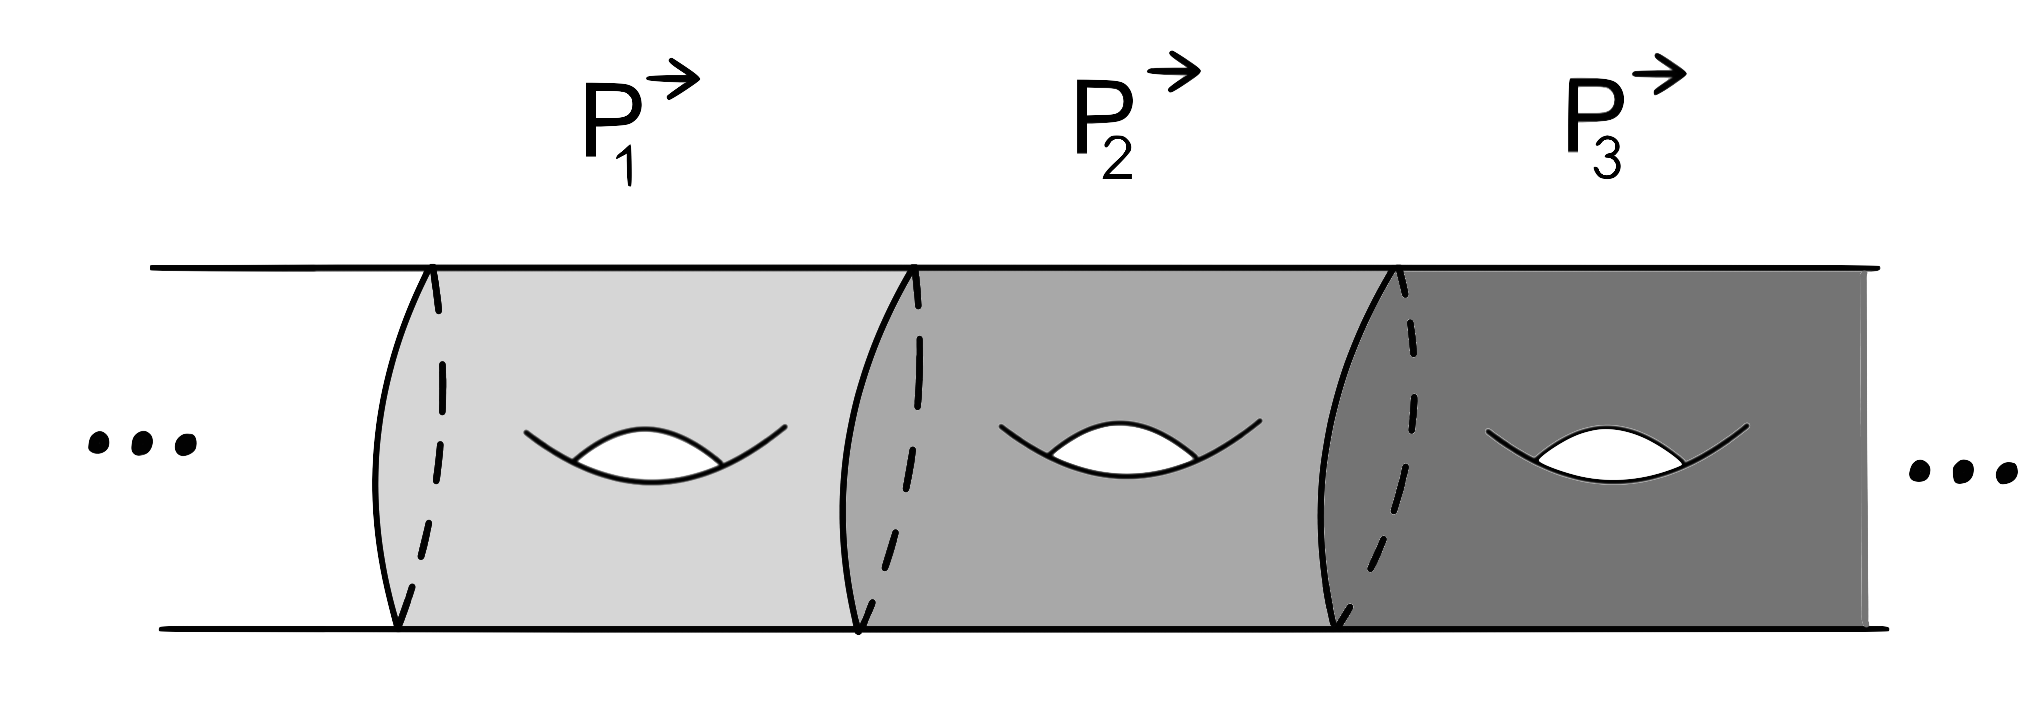
\includegraphics[width=2in,height=0.7in]{imagenes/final.png} 
\end{center}
\end{figure}

\begin{defi}
El borde ideal $B(S)$ de una superficie es el conjunto de extremos salvo equivalencia.
\end{defi}

\end{frame}

%%%%%% DIAPOSITIVA 14 %%%%%%
\begin{frame}
\frametitle{Topología de $B(S)$}
Sobre $B(S)$ tomamos la topología que tiene por base el conjunto \[\{U^*: U\subset S \text{, no acotado de frontera compacta}\}\]donde $U^*$ es el conjunto de extremos contenidos en $U$.
\begin{figure}[htb]
\begin{center}
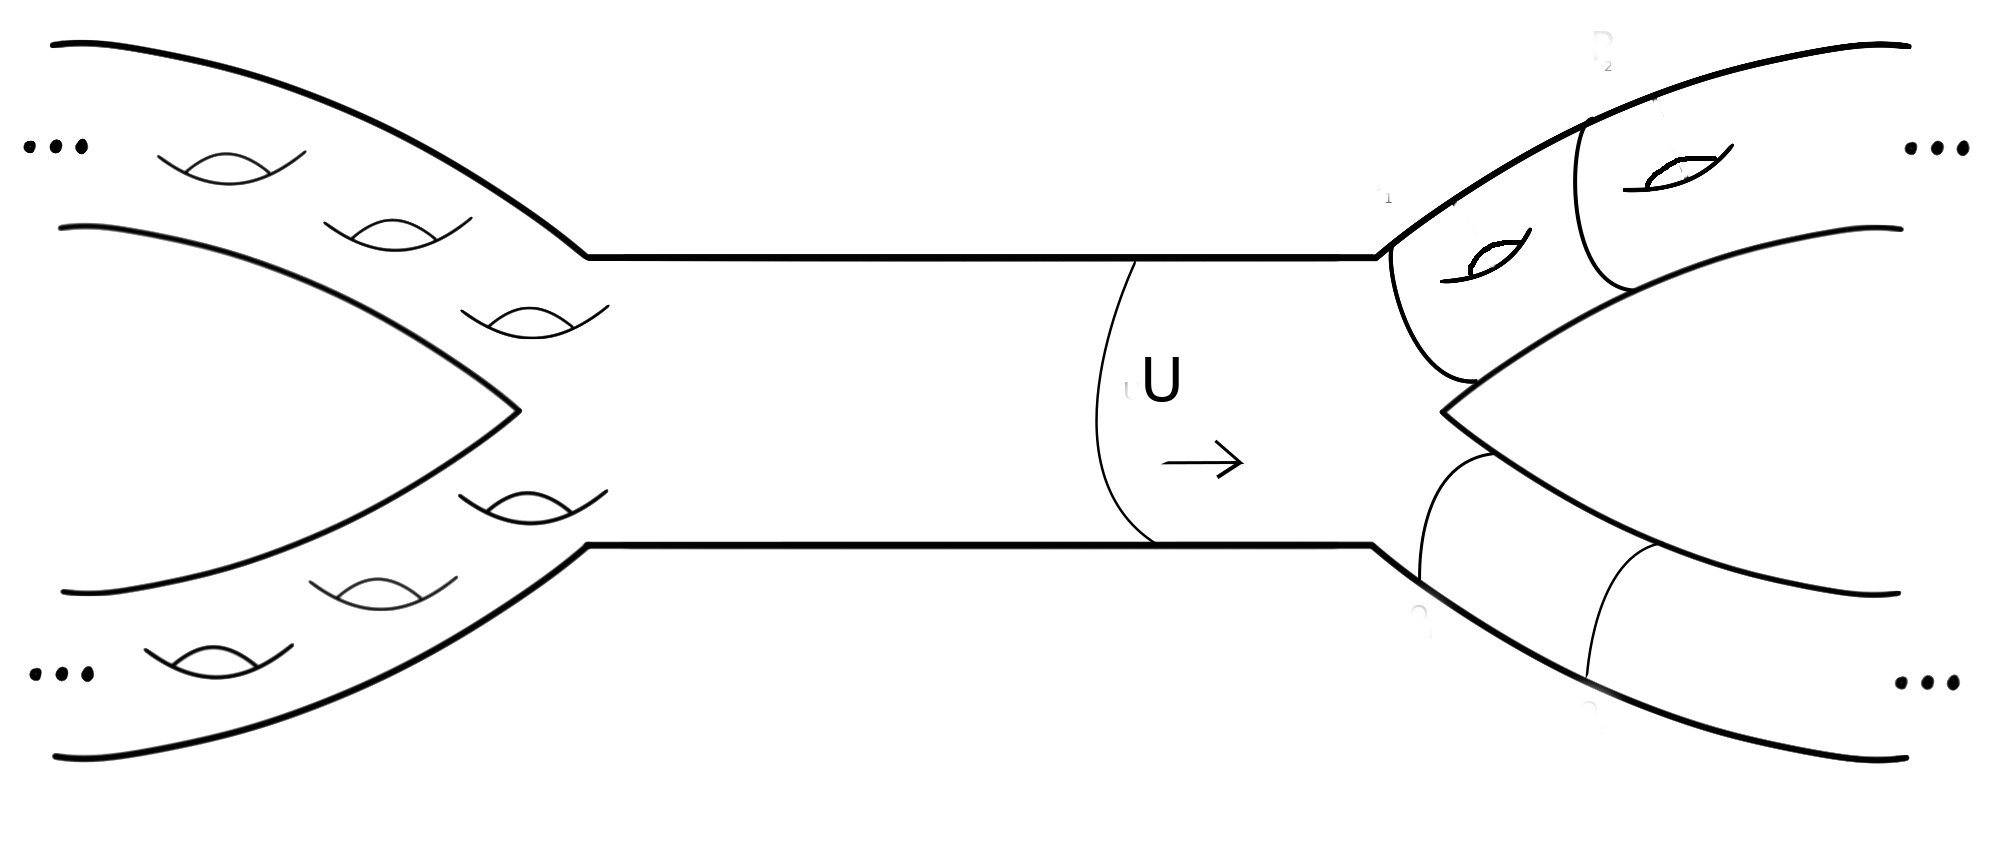
\includegraphics[width=2.5in,height=0.75in]{imagenes/diapoX.png} 
\end{center}
\end{figure}

El subconjunto de extremos de género infinito se denota por $B'(S)$. Se suele llamar borde ideal a la tupla $(B(S), B'(S))$.
\end{frame}
 

%%%%%% DIAPOSITIVA 15 %%%%%%
\begin{frame}
\frametitle{Teorema de clasificación de superficies no compactas}

\begin{teor}
Sean $S$ y $S'$ dos superficies orientables del mismo género, entonces serán homeomorfas si y solo si lo son sus bordes ideales como tuplas de espacios.
\end{teor}

\begin{proof}[Demostración]
El homeomorfismo entre bordes ideales nos permite definir las sucesiones de subsuperficies compactas $A_1 \subset A_2 \subset ...$ y $A'_1 \subset A'_2 \subset ...$ de modo que:
\begin{itemize}
\item Recubren a $S$ y $S'$, respectivamente.
\item Para todo $n$ existe el homeomorfismo entre subsuperficies $f_n: A_n \longrightarrow A'_n$.
\end{itemize} 
El homeomorfismo entre las superficies $S$ y $S'$ será $f = \lim_{n\to\infty} f_n$.

\end{proof}

\end{frame}


\begin{frame}
\frametitle{Representantes de superficies no compactas.}


\begin{prop}
El borde ideal de una superficie $(B(S), B'(S))$ es homeomorfo a $(X,Y)$ con $Y$ cerrado de $X$, y $X$ un subconjunto cerrado del conjunto de Cantor.
\end{prop}

\begin{teor}
Para todo par $(X,Y)$ anterior, podemos construir una superficie con ese borde ideal.
\end{teor}


\end{frame}




\begin{frame}
\frametitle{Cardinalidad}
Cardinalidad de superficies salvo homeomorfismo:
\begin{itemize}
\item Hay $\aleph_0$ superficies compactas
\begin{figure}[htb]
\begin{center}
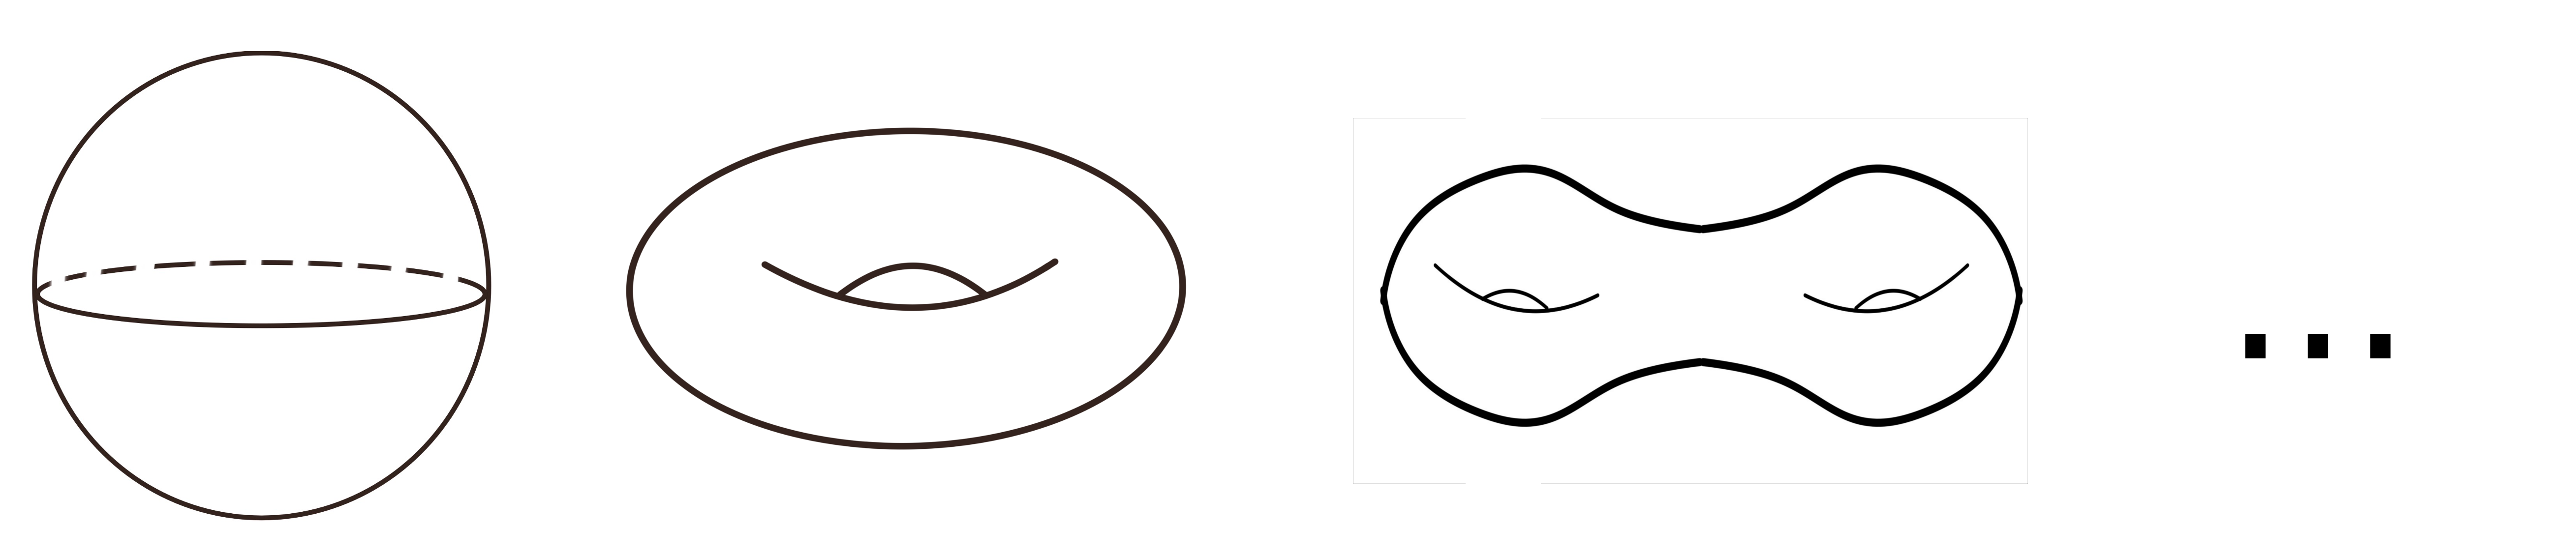
\includegraphics[width=4in,height=0.75in]{imagenes/diapo4.png} 
\end{center}
\end{figure}

\item Hay $\aleph_1$ superficies no compactas (cantidad de subconjuntos cerrados del conjuntos de Cantor no homeomorfos entre sí).

\item  Hay $\aleph_2$ superficies \textbf{no} segundo numerables.
\end{itemize}



\end{frame}

 

 
 
 
 
\end{document}




